\documentclass{standalone}
\usepackage{tikz}
\usetikzlibrary{patterns, positioning}


\begin{document}
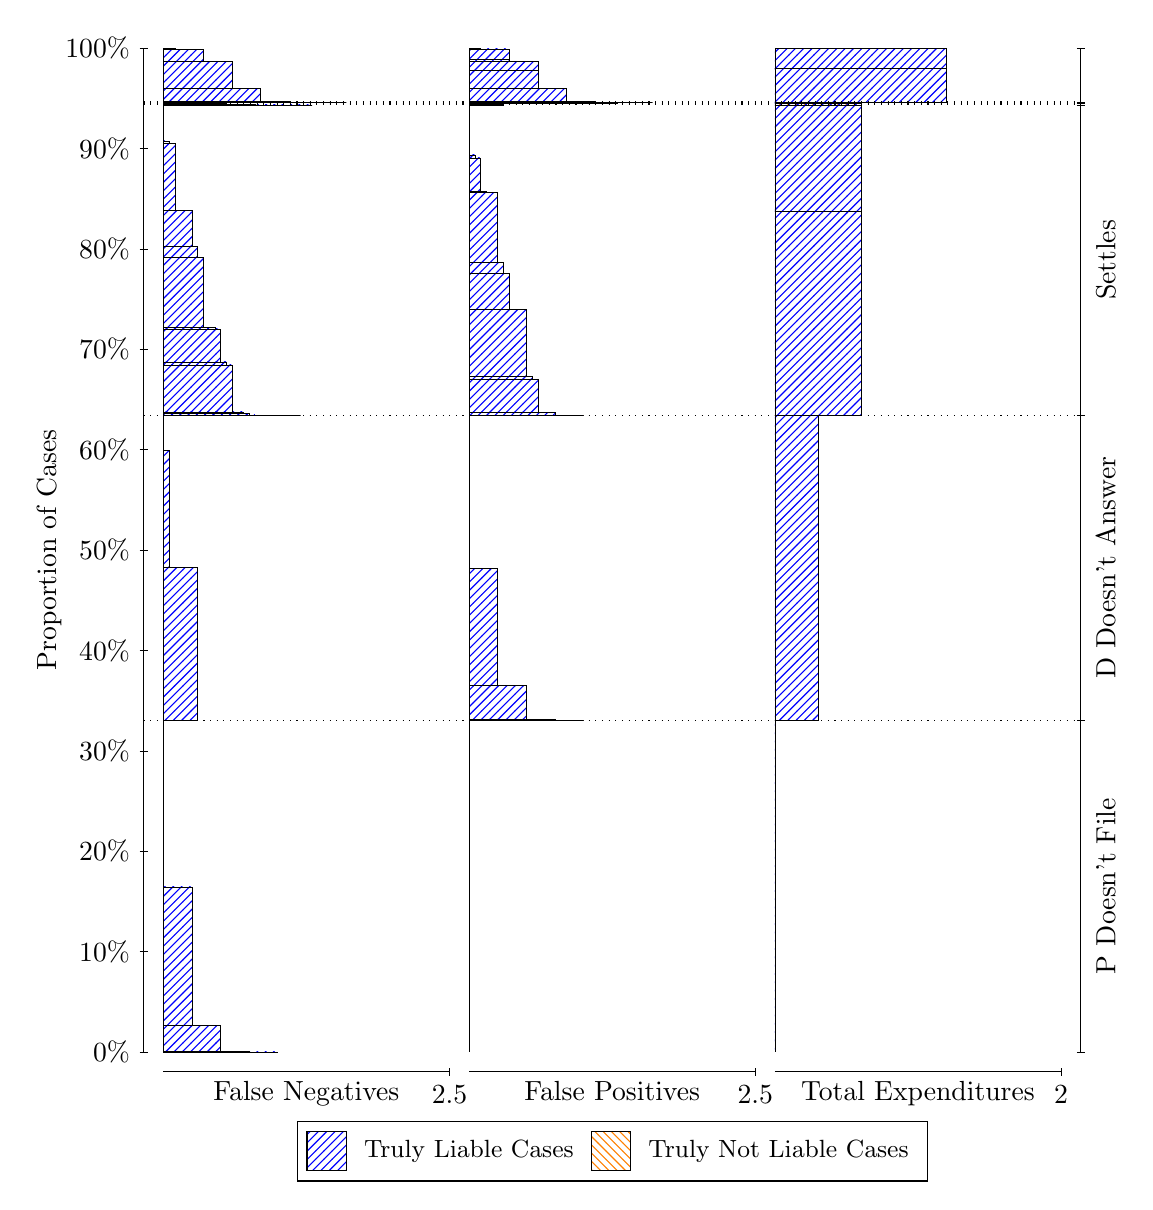
\begin{tikzpicture}
\draw[black, very thin] (1.5,1.75) -- (1.5,14.5);
\node[rotate=90, text=black, anchor=center] at (0.3, 8.125) {Proportion of Cases};
\draw[black, very thin] (1.45,1.75) -- (1.55,1.75);
\node[text=black, anchor=east] at (1.45, 1.75) {0\%};
\draw[black, very thin] (1.45,3.025) -- (1.55,3.025);
\node[text=black, anchor=east] at (1.45, 3.025) {10\%};
\draw[black, very thin] (1.45,4.3) -- (1.55,4.3);
\node[text=black, anchor=east] at (1.45, 4.3) {20\%};
\draw[black, very thin] (1.45,5.575) -- (1.55,5.575);
\node[text=black, anchor=east] at (1.45, 5.575) {30\%};
\draw[black, very thin] (1.45,6.85) -- (1.55,6.85);
\node[text=black, anchor=east] at (1.45, 6.85) {40\%};
\draw[black, very thin] (1.45,8.125) -- (1.55,8.125);
\node[text=black, anchor=east] at (1.45, 8.125) {50\%};
\draw[black, very thin] (1.45,9.4) -- (1.55,9.4);
\node[text=black, anchor=east] at (1.45, 9.4) {60\%};
\draw[black, very thin] (1.45,10.675) -- (1.55,10.675);
\node[text=black, anchor=east] at (1.45, 10.675) {70\%};
\draw[black, very thin] (1.45,11.95) -- (1.55,11.95);
\node[text=black, anchor=east] at (1.45, 11.95) {80\%};
\draw[black, very thin] (1.45,13.225) -- (1.55,13.225);
\node[text=black, anchor=east] at (1.45, 13.225) {90\%};
\draw[black, very thin] (1.45,14.5) -- (1.55,14.5);
\node[text=black, anchor=east] at (1.45, 14.5) {100\%};

\draw[black, very thin] (13.4,1.75) -- (13.4,14.5);
\draw[black, very thin] (13.35,1.75) -- (13.45,1.75);
\node[anchor=west] at (13.35, 1.75) {};
\draw[black, very thin] (13.35,5.9619) -- (13.45,5.9619);
\node[anchor=west] at (13.35, 5.9619) {};
\draw[black, very thin] (13.35,9.8382) -- (13.45,9.8382);
\node[anchor=west] at (13.35, 9.8382) {};
\draw[black, very thin] (13.35,13.779) -- (13.45,13.779);
\node[anchor=west] at (13.35, 13.779) {};
\draw[black, very thin] (13.35,13.8) -- (13.45,13.8);
\node[anchor=west] at (13.35, 13.8) {};
\draw[black, very thin] (13.35,13.814) -- (13.45,13.814);
\node[anchor=west] at (13.35, 13.814) {};
\draw[black, very thin] (13.35,14.5) -- (13.45,14.5);
\node[anchor=west] at (13.35, 14.5) {};

\draw[black, very thin, pattern color=blue, pattern=north east lines] (1.75,1.75) rectangle (3.2033,1.75);
\draw[black, very thin, pattern color=blue, pattern=north east lines] (1.75,1.75) rectangle (2.84,1.7528);
\draw[black, very thin, pattern color=blue, pattern=north east lines] (1.75,1.7528) rectangle (2.4767,2.0843);
\draw[black, very thin, pattern color=blue, pattern=north east lines] (1.75,2.0843) rectangle (2.1133,3.847);
\draw[black, very thin, pattern color=orange, pattern=north west lines] (1.75,3.847) rectangle (1.75,3.847);
\draw[black, very thin, pattern color=blue, pattern=north east lines] (1.75,3.847) rectangle (1.75,5.9619);
\draw[black, very thin, pattern color=blue, pattern=north east lines] (1.75,5.9619) rectangle (2.186,7.9076);
\draw[black, very thin, pattern color=blue, pattern=north east lines] (1.75,7.9076) rectangle (1.8227,9.3928);
\draw[black, very thin, pattern color=orange, pattern=north west lines] (1.75,9.3928) rectangle (1.75,9.3928);
\draw[black, very thin, pattern color=blue, pattern=north east lines] (1.75,9.3928) rectangle (1.75,9.8382);
\draw[black, very thin, pattern color=blue, pattern=north east lines] (1.75,9.8382) rectangle (3.494,9.8382);
\draw[black, very thin, pattern color=blue, pattern=north east lines] (1.75,9.8382) rectangle (3.2033,9.8382);
\draw[black, very thin, pattern color=blue, pattern=north east lines] (1.75,9.8382) rectangle (3.1307,9.8387);
\draw[black, very thin, pattern color=blue, pattern=north east lines] (1.75,9.8387) rectangle (2.9127,9.8397);
\draw[black, very thin, pattern color=blue, pattern=north east lines] (1.75,9.8397) rectangle (2.84,9.8557);
\draw[black, very thin, pattern color=blue, pattern=north east lines] (1.75,9.8557) rectangle (2.7673,9.8786);
\draw[black, very thin, pattern color=blue, pattern=north east lines] (1.75,9.8786) rectangle (2.622,10.475);
\draw[black, very thin, pattern color=blue, pattern=north east lines] (1.75,10.475) rectangle (2.5493,10.513);
\draw[black, very thin, pattern color=blue, pattern=north east lines] (1.75,10.513) rectangle (2.4767,10.934);
\draw[black, very thin, pattern color=blue, pattern=north east lines] (1.75,10.934) rectangle (2.404,10.951);
\draw[black, very thin, pattern color=blue, pattern=north east lines] (1.75,10.951) rectangle (2.2587,11.842);
\draw[black, very thin, pattern color=blue, pattern=north east lines] (1.75,11.842) rectangle (2.186,11.984);
\draw[black, very thin, pattern color=blue, pattern=north east lines] (1.75,11.984) rectangle (2.1133,12.435);
\draw[black, very thin, pattern color=blue, pattern=north east lines] (1.75,12.435) rectangle (2.0407,12.435);
\draw[black, very thin, pattern color=blue, pattern=north east lines] (1.75,12.435) rectangle (1.8953,13.286);
\draw[black, very thin, pattern color=blue, pattern=north east lines] (1.75,13.286) rectangle (1.8227,13.321);
\draw[black, very thin, pattern color=orange, pattern=north west lines] (1.75,13.321) rectangle (1.75,13.321);
\draw[black, very thin, pattern color=blue, pattern=north east lines] (1.75,13.321) rectangle (1.75,13.779);
\draw[black, very thin, pattern color=blue, pattern=north east lines] (1.75,13.779) rectangle (3.6393,13.779);
\draw[black, very thin, pattern color=blue, pattern=north east lines] (1.75,13.779) rectangle (3.276,13.779);
\draw[black, very thin, pattern color=blue, pattern=north east lines] (1.75,13.779) rectangle (2.9127,13.781);
\draw[black, very thin, pattern color=blue, pattern=north east lines] (1.75,13.781) rectangle (2.5493,13.794);
\draw[black, very thin, pattern color=blue, pattern=north east lines] (1.75,13.794) rectangle (2.186,13.8);
\draw[black, very thin, pattern color=orange, pattern=north west lines] (1.75,13.8) rectangle (1.75,13.8);
\draw[black, very thin, pattern color=blue, pattern=north east lines] (1.75,13.8) rectangle (2.186,13.806);
\draw[black, very thin, pattern color=blue, pattern=north east lines] (1.75,13.806) rectangle (1.8227,13.814);
\draw[black, very thin, pattern color=orange, pattern=north west lines] (1.75,13.814) rectangle (1.75,13.814);
\draw[black, very thin, pattern color=blue, pattern=north east lines] (1.75,13.814) rectangle (1.75,13.814);
\draw[black, very thin, pattern color=blue, pattern=north east lines] (1.75,13.814) rectangle (4.0753,13.814);
\draw[black, very thin, pattern color=blue, pattern=north east lines] (1.75,13.814) rectangle (3.712,13.814);
\draw[black, very thin, pattern color=blue, pattern=north east lines] (1.75,13.814) rectangle (3.3487,13.825);
\draw[black, very thin, pattern color=blue, pattern=north east lines] (1.75,13.825) rectangle (2.9853,13.983);
\draw[black, very thin, pattern color=blue, pattern=north east lines] (1.75,13.983) rectangle (2.622,14.328);
\draw[black, very thin, pattern color=blue, pattern=north east lines] (1.75,14.328) rectangle (2.2587,14.487);
\draw[black, very thin, pattern color=blue, pattern=north east lines] (1.75,14.487) rectangle (1.8953,14.5);
\draw[black, very thin, pattern color=orange, pattern=north west lines] (1.75,14.5) rectangle (1.75,14.5);
\draw[black, very thin, pattern color=blue, pattern=north east lines] (1.75,14.5) rectangle (1.75,14.5);
\draw[black, very thin, pattern color=orange, pattern=north west lines] (5.6333,1.75) rectangle (5.6333,1.75);
\draw[black, very thin, pattern color=blue, pattern=north east lines] (5.6333,1.75) rectangle (5.6333,5.9619);
\draw[black, very thin, pattern color=orange, pattern=north west lines] (5.6333,5.9619) rectangle (7.0867,5.9619);
\draw[black, very thin, pattern color=blue, pattern=north east lines] (5.6333,5.9619) rectangle (7.0867,5.9619);
\draw[black, very thin, pattern color=blue, pattern=north east lines] (5.6333,5.9619) rectangle (6.7233,5.9718);
\draw[black, very thin, pattern color=blue, pattern=north east lines] (5.6333,5.9718) rectangle (6.36,6.4074);
\draw[black, very thin, pattern color=blue, pattern=north east lines] (5.6333,6.4074) rectangle (5.9967,7.8925);
\draw[black, very thin, pattern color=blue, pattern=north east lines] (5.6333,7.8925) rectangle (5.6333,9.8382);
\draw[black, very thin, pattern color=orange, pattern=north west lines] (5.6333,9.8382) rectangle (7.0867,9.8382);
\draw[black, very thin, pattern color=blue, pattern=north east lines] (5.6333,9.8382) rectangle (7.0867,9.8382);
\draw[black, very thin, pattern color=orange, pattern=north west lines] (5.6333,9.8382) rectangle (6.796,9.8382);
\draw[black, very thin, pattern color=blue, pattern=north east lines] (5.6333,9.8382) rectangle (6.796,9.8391);
\draw[black, very thin, pattern color=blue, pattern=north east lines] (5.6333,9.8391) rectangle (6.7233,9.8712);
\draw[black, very thin, pattern color=orange, pattern=north west lines] (5.6333,9.8712) rectangle (6.5053,9.8712);
\draw[black, very thin, pattern color=blue, pattern=north east lines] (5.6333,9.8712) rectangle (6.5053,10.296);
\draw[black, very thin, pattern color=blue, pattern=north east lines] (5.6333,10.296) rectangle (6.4327,10.332);
\draw[black, very thin, pattern color=blue, pattern=north east lines] (5.6333,10.332) rectangle (6.36,11.183);
\draw[black, very thin, pattern color=orange, pattern=north west lines] (5.6333,11.183) rectangle (6.2147,11.183);
\draw[black, very thin, pattern color=blue, pattern=north east lines] (5.6333,11.183) rectangle (6.2147,11.183);
\draw[black, very thin, pattern color=blue, pattern=north east lines] (5.6333,11.183) rectangle (6.142,11.634);
\draw[black, very thin, pattern color=blue, pattern=north east lines] (5.6333,11.634) rectangle (6.0693,11.776);
\draw[black, very thin, pattern color=blue, pattern=north east lines] (5.6333,11.776) rectangle (5.9967,12.666);
\draw[black, very thin, pattern color=blue, pattern=north east lines] (5.6333,12.666) rectangle (5.8513,12.684);
\draw[black, very thin, pattern color=blue, pattern=north east lines] (5.6333,12.684) rectangle (5.7787,13.105);
\draw[black, very thin, pattern color=blue, pattern=north east lines] (5.6333,13.105) rectangle (5.706,13.143);
\draw[black, very thin, pattern color=blue, pattern=north east lines] (5.6333,13.143) rectangle (5.6333,13.779);
\draw[black, very thin, pattern color=orange, pattern=north west lines] (5.6333,13.779) rectangle (6.0693,13.779);
\draw[black, very thin, pattern color=blue, pattern=north east lines] (5.6333,13.779) rectangle (6.0693,13.786);
\draw[black, very thin, pattern color=blue, pattern=north east lines] (5.6333,13.786) rectangle (5.706,13.799);
\draw[black, very thin, pattern color=blue, pattern=north east lines] (5.6333,13.799) rectangle (5.6333,13.8);
\draw[black, very thin, pattern color=orange, pattern=north west lines] (5.6333,13.8) rectangle (7.5227,13.8);
\draw[black, very thin, pattern color=blue, pattern=north east lines] (5.6333,13.8) rectangle (7.5227,13.8);
\draw[black, very thin, pattern color=blue, pattern=north east lines] (5.6333,13.8) rectangle (7.1593,13.8);
\draw[black, very thin, pattern color=blue, pattern=north east lines] (5.6333,13.8) rectangle (6.796,13.8);
\draw[black, very thin, pattern color=blue, pattern=north east lines] (5.6333,13.8) rectangle (6.4327,13.809);
\draw[black, very thin, pattern color=blue, pattern=north east lines] (5.6333,13.809) rectangle (6.0693,13.814);
\draw[black, very thin, pattern color=orange, pattern=north west lines] (5.6333,13.814) rectangle (7.9587,13.814);
\draw[black, very thin, pattern color=blue, pattern=north east lines] (5.6333,13.814) rectangle (7.9587,13.814);
\draw[black, very thin, pattern color=orange, pattern=north west lines] (5.6333,13.814) rectangle (7.5953,13.814);
\draw[black, very thin, pattern color=blue, pattern=north east lines] (5.6333,13.814) rectangle (7.5953,13.814);
\draw[black, very thin, pattern color=orange, pattern=north west lines] (5.6333,13.814) rectangle (7.232,13.814);
\draw[black, very thin, pattern color=blue, pattern=north east lines] (5.6333,13.814) rectangle (7.232,13.827);
\draw[black, very thin, pattern color=blue, pattern=north east lines] (5.6333,13.827) rectangle (6.8687,13.986);
\draw[black, very thin, pattern color=orange, pattern=north west lines] (5.6333,13.986) rectangle (6.8687,13.986);
\draw[black, very thin, pattern color=blue, pattern=north east lines] (5.6333,13.986) rectangle (6.8687,13.987);
\draw[black, very thin, pattern color=blue, pattern=north east lines] (5.6333,13.987) rectangle (6.5053,14.213);
\draw[black, very thin, pattern color=orange, pattern=north west lines] (5.6333,14.213) rectangle (6.5053,14.213);
\draw[black, very thin, pattern color=blue, pattern=north east lines] (5.6333,14.213) rectangle (6.5053,14.331);
\draw[black, very thin, pattern color=blue, pattern=north east lines] (5.6333,14.331) rectangle (6.142,14.357);
\draw[black, very thin, pattern color=blue, pattern=north east lines] (5.6333,14.357) rectangle (6.142,14.49);
\draw[black, very thin, pattern color=blue, pattern=north east lines] (5.6333,14.49) rectangle (5.7787,14.49);
\draw[black, very thin, pattern color=blue, pattern=north east lines] (5.6333,14.49) rectangle (5.7787,14.5);
\draw[black, very thin, pattern color=blue, pattern=north east lines] (5.6333,14.5) rectangle (5.6333,14.5);
\draw[black, very thin, pattern color=orange, pattern=north west lines] (9.5167,1.75) rectangle (9.5167,1.75);
\draw[black, very thin, pattern color=blue, pattern=north east lines] (9.5167,1.75) rectangle (9.5167,5.9619);
\draw[black, very thin, pattern color=orange, pattern=north west lines] (9.5167,5.9619) rectangle (10.062,5.9619);
\draw[black, very thin, pattern color=blue, pattern=north east lines] (9.5167,5.9619) rectangle (10.062,9.8382);
\draw[black, very thin, pattern color=orange, pattern=north west lines] (9.5167,9.8382) rectangle (10.607,9.8382);
\draw[black, very thin, pattern color=blue, pattern=north east lines] (9.5167,9.8382) rectangle (10.607,12.425);
\draw[black, very thin, pattern color=orange, pattern=north west lines] (9.5167,12.425) rectangle (10.607,12.425);
\draw[black, very thin, pattern color=blue, pattern=north east lines] (9.5167,12.425) rectangle (10.607,13.779);
\draw[black, very thin, pattern color=orange, pattern=north west lines] (9.5167,13.779) rectangle (10.607,13.779);
\draw[black, very thin, pattern color=blue, pattern=north east lines] (9.5167,13.779) rectangle (10.607,13.8);
\draw[black, very thin, pattern color=orange, pattern=north west lines] (9.5167,13.8) rectangle (10.607,13.8);
\draw[black, very thin, pattern color=blue, pattern=north east lines] (9.5167,13.8) rectangle (10.607,13.814);
\draw[black, very thin, pattern color=orange, pattern=north west lines] (9.5167,13.814) rectangle (11.697,13.814);
\draw[black, very thin, pattern color=blue, pattern=north east lines] (9.5167,13.814) rectangle (11.697,14.238);
\draw[black, very thin, pattern color=orange, pattern=north west lines] (9.5167,14.238) rectangle (11.697,14.238);
\draw[black, very thin, pattern color=blue, pattern=north east lines] (9.5167,14.238) rectangle (11.697,14.5);
\draw[black, dotted] (1.5,5.9619) -- (13.4,5.9619);
\draw[black, dotted] (1.5,9.8382) -- (13.4,9.8382);
\draw[black, dotted] (1.5,13.779) -- (13.4,13.779);
\draw[black, dotted] (1.5,13.8) -- (13.4,13.8);
\draw[black, dotted] (1.5,13.814) -- (13.4,13.814);
\draw[black, very thin] (1.75,1.5) -- (5.3833,1.5);
\node[text=black, anchor=north] at (3.5667, 1.5) {False Negatives};
\draw[black, very thin] (5.3833,1.45) -- (5.3833,1.55);
\node[text=black, anchor=north] at (5.3833, 1.45) {2.5};

\draw[black, very thin] (5.6333,1.5) -- (9.2667,1.5);
\node[text=black, anchor=north] at (7.45, 1.5) {False Positives};
\draw[black, very thin] (9.2667,1.45) -- (9.2667,1.55);
\node[text=black, anchor=north] at (9.2667, 1.45) {2.5};

\draw[black, very thin] (9.5167,1.5) -- (13.15,1.5);
\node[text=black, anchor=north] at (11.333, 1.5) {Total Expenditures};
\draw[black, very thin] (13.15,1.45) -- (13.15,1.55);
\node[text=black, anchor=north] at (13.15, 1.45) {2};

\node[text=black, centered, rotate=90] at (13.72, 3.8559) {P Doesn't File};
\node[text=black, centered, rotate=90] at (13.72, 7.9001) {D Doesn't Answer};
\node[text=black, centered, rotate=90] at (13.72, 11.809) {Settles};




\draw (7.449999999999999,1.5) node[draw=none] (baseCoordinate) {};
\begin{scope}[align=center]
        \matrix[scale=0.5, draw=black, below=0.5cm of baseCoordinate, nodes={draw}, column sep=0.1cm]{
            \node[rectangle, draw, minimum width=0.5cm, minimum height=0.5cm, pattern color=blue, pattern=north east lines] {}; &
            \node[draw=none, font=\small, text=black] (B) {Truly Liable Cases}; &
            \node[rectangle, draw, minimum width=0.5cm, minimum height=0.5cm, pattern color=orange, pattern=north west lines] {}; &
            \node[draw=none, font=\small, text=black] (B) {Truly Not Liable Cases}; \\
            };
\end{scope}

\end{tikzpicture}
\end{document}